\documentclass[twoside]{book}

% Packages required by doxygen
\usepackage{fixltx2e}
\usepackage{calc}
\usepackage{doxygen}
\usepackage{graphicx}
\usepackage[utf8]{inputenc}
\usepackage{makeidx}
\usepackage{multicol}
\usepackage{multirow}
\PassOptionsToPackage{warn}{textcomp}
\usepackage{textcomp}
\usepackage[nointegrals]{wasysym}
\usepackage[table]{xcolor}

% Font selection
\usepackage[T1]{fontenc}
\usepackage{mathptmx}
\usepackage[scaled=.90]{helvet}
\usepackage{courier}
\usepackage{amssymb}
\usepackage{sectsty}
\renewcommand{\familydefault}{\sfdefault}
\allsectionsfont{%
  \fontseries{bc}\selectfont%
  \color{darkgray}%
}
\renewcommand{\DoxyLabelFont}{%
  \fontseries{bc}\selectfont%
  \color{darkgray}%
}
\newcommand{\+}{\discretionary{\mbox{\scriptsize$\hookleftarrow$}}{}{}}

% Page & text layout
\usepackage{geometry}
\geometry{%
  a4paper,%
  top=2.5cm,%
  bottom=2.5cm,%
  left=2.5cm,%
  right=2.5cm%
}
\tolerance=750
\hfuzz=15pt
\hbadness=750
\setlength{\emergencystretch}{15pt}
\setlength{\parindent}{0cm}
\setlength{\parskip}{0.2cm}
\makeatletter
\renewcommand{\paragraph}{%
  \@startsection{paragraph}{4}{0ex}{-1.0ex}{1.0ex}{%
    \normalfont\normalsize\bfseries\SS@parafont%
  }%
}
\renewcommand{\subparagraph}{%
  \@startsection{subparagraph}{5}{0ex}{-1.0ex}{1.0ex}{%
    \normalfont\normalsize\bfseries\SS@subparafont%
  }%
}
\makeatother

% Headers & footers
\usepackage{fancyhdr}
\pagestyle{fancyplain}
\fancyhead[LE]{\fancyplain{}{\bfseries\thepage}}
\fancyhead[CE]{\fancyplain{}{}}
\fancyhead[RE]{\fancyplain{}{\bfseries\leftmark}}
\fancyhead[LO]{\fancyplain{}{\bfseries\rightmark}}
\fancyhead[CO]{\fancyplain{}{}}
\fancyhead[RO]{\fancyplain{}{\bfseries\thepage}}
\fancyfoot[LE]{\fancyplain{}{}}
\fancyfoot[CE]{\fancyplain{}{}}
\fancyfoot[RE]{\fancyplain{}{\bfseries\scriptsize Generated on Sun Oct 26 2014 20\+:16\+:38 for Bored\+Room\+Bingo by Doxygen }}
\fancyfoot[LO]{\fancyplain{}{\bfseries\scriptsize Generated on Sun Oct 26 2014 20\+:16\+:38 for Bored\+Room\+Bingo by Doxygen }}
\fancyfoot[CO]{\fancyplain{}{}}
\fancyfoot[RO]{\fancyplain{}{}}
\renewcommand{\footrulewidth}{0.4pt}
\renewcommand{\chaptermark}[1]{%
  \markboth{#1}{}%
}
\renewcommand{\sectionmark}[1]{%
  \markright{\thesection\ #1}%
}

% Indices & bibliography
\usepackage{natbib}
\usepackage[titles]{tocloft}
\setcounter{tocdepth}{3}
\setcounter{secnumdepth}{5}
\makeindex

% Hyperlinks (required, but should be loaded last)
\usepackage{ifpdf}
\ifpdf
  \usepackage[pdftex,pagebackref=true]{hyperref}
\else
  \usepackage[ps2pdf,pagebackref=true]{hyperref}
\fi
\hypersetup{%
  colorlinks=true,%
  linkcolor=blue,%
  citecolor=blue,%
  unicode%
}

% Custom commands
\newcommand{\clearemptydoublepage}{%
  \newpage{\pagestyle{empty}\cleardoublepage}%
}


%===== C O N T E N T S =====

\begin{document}

% Titlepage & ToC
\hypersetup{pageanchor=false,
             bookmarks=true,
             bookmarksnumbered=true,
             pdfencoding=unicode
            }
\pagenumbering{roman}
\begin{titlepage}
\vspace*{7cm}
\begin{center}%
{\Large Bored\+Room\+Bingo }\\
\vspace*{1cm}
{\large Generated by Doxygen 1.8.8}\\
\vspace*{0.5cm}
{\small Sun Oct 26 2014 20:16:38}\\
\end{center}
\end{titlepage}
\clearemptydoublepage
\tableofcontents
\clearemptydoublepage
\pagenumbering{arabic}
\hypersetup{pageanchor=true}

%--- Begin generated contents ---
\chapter{Hierarchical Index}
\section{Class Hierarchy}
This inheritance list is sorted roughly, but not completely, alphabetically\+:\begin{DoxyCompactList}
\item \contentsline{section}{App\+Delegate()}{\pageref{category_app_delegate_07_08}}{}
\item \contentsline{section}{Archived\+Word\+Lists\+Table\+View\+Controller()}{\pageref{category_archived_word_lists_table_view_controller_07_08}}{}
\item \contentsline{section}{Bingo\+Board\+View\+Controller()}{\pageref{category_bingo_board_view_controller_07_08}}{}
\item \contentsline{section}{Chat\+View\+Controller()}{\pageref{category_chat_view_controller_07_08}}{}
\item \contentsline{section}{Current\+Words\+Table\+View\+Controller()}{\pageref{category_current_words_table_view_controller_07_08}}{}
\item \contentsline{section}{Detail\+Archive\+Wordlist\+Table\+View\+Controller()}{\pageref{category_detail_archive_wordlist_table_view_controller_07_08}}{}
\item $<$F\+B\+Login\+View\+Delegate$>$\begin{DoxyCompactList}
\item \contentsline{section}{Login\+Sign\+Up}{\pageref{interface_login_sign_up}}{}
\end{DoxyCompactList}
\item \contentsline{section}{Game\+Creation\+View\+Controller()}{\pageref{category_game_creation_view_controller_07_08}}{}
\item \contentsline{section}{Home\+Screen\+View\+Controller()}{\pageref{category_home_screen_view_controller_07_08}}{}
\item \contentsline{section}{Invite\+Friends\+View\+Controller()}{\pageref{category_invite_friends_view_controller_07_08}}{}
\item \contentsline{section}{M\+B\+Progress\+H\+U\+D()}{\pageref{category_m_b_progress_h_u_d_07_08}}{}
\item N\+S\+Error\begin{DoxyCompactList}
\item \contentsline{section}{Login\+Error}{\pageref{interface_login_error}}{}
\begin{DoxyCompactList}
\item \contentsline{section}{Default\+Error}{\pageref{interface_default_error}}{}
\item \contentsline{section}{Email\+Taken\+Error}{\pageref{interface_email_taken_error}}{}
\item \contentsline{section}{Invalid\+Email\+Error}{\pageref{interface_invalid_email_error}}{}
\item \contentsline{section}{Invalid\+Password\+Error}{\pageref{interface_invalid_password_error}}{}
\item \contentsline{section}{Network\+Error}{\pageref{interface_network_error}}{}
\item \contentsline{section}{User\+Does\+Not\+Exist\+Error}{\pageref{interface_user_does_not_exist_error}}{}
\end{DoxyCompactList}
\end{DoxyCompactList}
\item N\+S\+Object\begin{DoxyCompactList}
\item \contentsline{section}{Board\+Model}{\pageref{interface_board_model}}{}
\end{DoxyCompactList}
\item $<$N\+S\+Object$>$\begin{DoxyCompactList}
\item \contentsline{section}{$<$Invitations\+Table\+View\+Cell\+Delegate$>$}{\pageref{protocol_invitations_table_view_cell_delegate-p}}{}
\begin{DoxyCompactList}
\item \contentsline{section}{Invitations\+Table\+View\+Controller()}{\pageref{category_invitations_table_view_controller_07_08}}{}
\end{DoxyCompactList}
\end{DoxyCompactList}
\item \contentsline{section}{Public\+Games\+Table\+View\+Controller()}{\pageref{category_public_games_table_view_controller_07_08}}{}
\item \contentsline{section}{Search\+Users\+Table\+View\+Controller()}{\pageref{category_search_users_table_view_controller_07_08}}{}
\item $<$U\+I\+Alert\+View\+Delegate$>$\begin{DoxyCompactList}
\item \contentsline{section}{Bingo\+Board\+View\+Controller}{\pageref{interface_bingo_board_view_controller}}{}
\item \contentsline{section}{Forgot\+Password\+View\+Controller}{\pageref{interface_forgot_password_view_controller}}{}
\item \contentsline{section}{Login\+Sign\+Up}{\pageref{interface_login_sign_up}}{}
\end{DoxyCompactList}
\item $<$U\+I\+Application\+Delegate$>$\begin{DoxyCompactList}
\item \contentsline{section}{App\+Delegate}{\pageref{interface_app_delegate}}{}
\end{DoxyCompactList}
\item $<$U\+I\+Gesture\+Recognizer\+Delegate$>$\begin{DoxyCompactList}
\item \contentsline{section}{Game\+Creation\+View\+Controller}{\pageref{interface_game_creation_view_controller}}{}
\item \contentsline{section}{Invitation\+Table\+View\+Cell()}{\pageref{category_invitation_table_view_cell_07_08}}{}
\end{DoxyCompactList}
\item U\+I\+Responder\begin{DoxyCompactList}
\item \contentsline{section}{App\+Delegate}{\pageref{interface_app_delegate}}{}
\end{DoxyCompactList}
\item U\+I\+Table\+View\begin{DoxyCompactList}
\item \contentsline{section}{U\+I\+Touch\+Table\+View}{\pageref{interface_u_i_touch_table_view}}{}
\end{DoxyCompactList}
\item U\+I\+Table\+View\+Cell\begin{DoxyCompactList}
\item \contentsline{section}{Current\+Words\+Table\+View\+Cell}{\pageref{interface_current_words_table_view_cell}}{}
\item \contentsline{section}{Invitation\+Table\+View\+Cell}{\pageref{interface_invitation_table_view_cell}}{}
\item \contentsline{section}{Search\+Users\+Table\+View\+Cell}{\pageref{interface_search_users_table_view_cell}}{}
\item \contentsline{section}{Select\+Word\+Table\+View\+Cell}{\pageref{interface_select_word_table_view_cell}}{}
\end{DoxyCompactList}
\item U\+I\+Table\+View\+Controller\begin{DoxyCompactList}
\item \contentsline{section}{Archived\+Word\+Lists\+Table\+View\+Controller}{\pageref{interface_archived_word_lists_table_view_controller}}{}
\item \contentsline{section}{Current\+Words\+Table\+View\+Controller}{\pageref{interface_current_words_table_view_controller}}{}
\item \contentsline{section}{Detail\+Archive\+Wordlist\+Table\+View\+Controller}{\pageref{interface_detail_archive_wordlist_table_view_controller}}{}
\item \contentsline{section}{Invitations\+Table\+View\+Controller}{\pageref{interface_invitations_table_view_controller}}{}
\item \contentsline{section}{Public\+Games\+Table\+View\+Controller}{\pageref{interface_public_games_table_view_controller}}{}
\item \contentsline{section}{Search\+Users\+Table\+View\+Controller}{\pageref{interface_search_users_table_view_controller}}{}
\end{DoxyCompactList}
\item $<$U\+I\+Table\+View\+Data\+Source$>$\begin{DoxyCompactList}
\item \contentsline{section}{Archived\+Word\+Lists\+Table\+View\+Controller}{\pageref{interface_archived_word_lists_table_view_controller}}{}
\item \contentsline{section}{Chat\+View\+Controller}{\pageref{interface_chat_view_controller}}{}
\end{DoxyCompactList}
\item $<$U\+I\+Table\+View\+Delegate$>$\begin{DoxyCompactList}
\item \contentsline{section}{Archived\+Word\+Lists\+Table\+View\+Controller}{\pageref{interface_archived_word_lists_table_view_controller}}{}
\item \contentsline{section}{Chat\+View\+Controller}{\pageref{interface_chat_view_controller}}{}
\end{DoxyCompactList}
\item $<$U\+I\+Text\+Field\+Delegate$>$\begin{DoxyCompactList}
\item \contentsline{section}{Game\+Creation\+View\+Controller}{\pageref{interface_game_creation_view_controller}}{}
\item \contentsline{section}{Invite\+Friends\+View\+Controller}{\pageref{interface_invite_friends_view_controller}}{}
\item \contentsline{section}{Login\+Sign\+Up}{\pageref{interface_login_sign_up}}{}
\end{DoxyCompactList}
\item U\+I\+View\begin{DoxyCompactList}
\item \contentsline{section}{M\+B\+Bar\+Progress\+View}{\pageref{interface_m_b_bar_progress_view}}{}
\item \contentsline{section}{M\+B\+Progress\+H\+U\+D}{\pageref{interface_m_b_progress_h_u_d}}{}
\item \contentsline{section}{M\+B\+Round\+Progress\+View}{\pageref{interface_m_b_round_progress_view}}{}
\end{DoxyCompactList}
\item U\+I\+View\+Controller\begin{DoxyCompactList}
\item \contentsline{section}{Bingo\+Board\+View\+Controller}{\pageref{interface_bingo_board_view_controller}}{}
\item \contentsline{section}{Chat\+View\+Controller}{\pageref{interface_chat_view_controller}}{}
\item \contentsline{section}{Error\+Message}{\pageref{interface_error_message}}{}
\item \contentsline{section}{Forgot\+Password\+View\+Controller}{\pageref{interface_forgot_password_view_controller}}{}
\item \contentsline{section}{Game\+Creation\+View\+Controller}{\pageref{interface_game_creation_view_controller}}{}
\item \contentsline{section}{Home\+Screen\+View\+Controller}{\pageref{interface_home_screen_view_controller}}{}
\item \contentsline{section}{Invite\+Friends\+View\+Controller}{\pageref{interface_invite_friends_view_controller}}{}
\item \contentsline{section}{Login\+Sign\+Up}{\pageref{interface_login_sign_up}}{}
\end{DoxyCompactList}
\item $<$U\+I\+View\+N\+S\+Object$>$\begin{DoxyCompactList}
\item \contentsline{section}{$<$M\+B\+Progress\+H\+U\+D\+Delegate$>$}{\pageref{protocol_m_b_progress_h_u_d_delegate-p}}{}
\end{DoxyCompactList}
\item X\+C\+Test\+Case\begin{DoxyCompactList}
\item \contentsline{section}{Login\+Sign\+Up\+Tests}{\pageref{interface_login_sign_up_tests}}{}
\end{DoxyCompactList}
\end{DoxyCompactList}

\chapter{Class Index}
\section{Class List}
Here are the classes, structs, unions and interfaces with brief descriptions\+:\begin{DoxyCompactList}
\item\contentsline{section}{\hyperlink{interface_app_delegate}{App\+Delegate} }{\pageref{interface_app_delegate}}{}
\item\contentsline{section}{\hyperlink{category_app_delegate_07_08}{App\+Delegate()} }{\pageref{category_app_delegate_07_08}}{}
\item\contentsline{section}{\hyperlink{interface_archived_word_lists_table_view_controller}{Archived\+Word\+Lists\+Table\+View\+Controller} }{\pageref{interface_archived_word_lists_table_view_controller}}{}
\item\contentsline{section}{\hyperlink{category_archived_word_lists_table_view_controller_07_08}{Archived\+Word\+Lists\+Table\+View\+Controller()} }{\pageref{category_archived_word_lists_table_view_controller_07_08}}{}
\item\contentsline{section}{\hyperlink{interface_bingo_board_view_controller}{Bingo\+Board\+View\+Controller} }{\pageref{interface_bingo_board_view_controller}}{}
\item\contentsline{section}{\hyperlink{category_bingo_board_view_controller_07_08}{Bingo\+Board\+View\+Controller()} }{\pageref{category_bingo_board_view_controller_07_08}}{}
\item\contentsline{section}{\hyperlink{interface_board_model}{Board\+Model} }{\pageref{interface_board_model}}{}
\item\contentsline{section}{\hyperlink{interface_current_words_table_view_cell}{Current\+Words\+Table\+View\+Cell} }{\pageref{interface_current_words_table_view_cell}}{}
\item\contentsline{section}{\hyperlink{interface_current_words_table_view_controller}{Current\+Words\+Table\+View\+Controller} }{\pageref{interface_current_words_table_view_controller}}{}
\item\contentsline{section}{\hyperlink{category_current_words_table_view_controller_07_08}{Current\+Words\+Table\+View\+Controller()} }{\pageref{category_current_words_table_view_controller_07_08}}{}
\item\contentsline{section}{\hyperlink{interface_detail_archive_wordlist_table_view_controller}{Detail\+Archive\+Wordlist\+Table\+View\+Controller} }{\pageref{interface_detail_archive_wordlist_table_view_controller}}{}
\item\contentsline{section}{\hyperlink{category_detail_archive_wordlist_table_view_controller_07_08}{Detail\+Archive\+Wordlist\+Table\+View\+Controller()} }{\pageref{category_detail_archive_wordlist_table_view_controller_07_08}}{}
\item\contentsline{section}{\hyperlink{interface_error_message}{Error\+Message} }{\pageref{interface_error_message}}{}
\item\contentsline{section}{\hyperlink{interface_forgot_password_view_controller}{Forgot\+Password\+View\+Controller} }{\pageref{interface_forgot_password_view_controller}}{}
\item\contentsline{section}{\hyperlink{interface_home_screen}{Home\+Screen} }{\pageref{interface_home_screen}}{}
\item\contentsline{section}{\hyperlink{category_home_screen_07_08}{Home\+Screen()} }{\pageref{category_home_screen_07_08}}{}
\item\contentsline{section}{\hyperlink{interface_login_sign_up}{Login\+Sign\+Up} }{\pageref{interface_login_sign_up}}{}
\item\contentsline{section}{\hyperlink{interface_login_sign_up_tests}{Login\+Sign\+Up\+Tests} }{\pageref{interface_login_sign_up_tests}}{}
\item\contentsline{section}{\hyperlink{interface_m_b_bar_progress_view}{M\+B\+Bar\+Progress\+View} }{\pageref{interface_m_b_bar_progress_view}}{}
\item\contentsline{section}{\hyperlink{interface_m_b_progress_h_u_d}{M\+B\+Progress\+H\+U\+D} }{\pageref{interface_m_b_progress_h_u_d}}{}
\item\contentsline{section}{\hyperlink{category_m_b_progress_h_u_d_07_08}{M\+B\+Progress\+H\+U\+D()} }{\pageref{category_m_b_progress_h_u_d_07_08}}{}
\item\contentsline{section}{\hyperlink{protocol_m_b_progress_h_u_d_delegate-p}{$<$\+M\+B\+Progress\+H\+U\+D\+Delegate$>$} }{\pageref{protocol_m_b_progress_h_u_d_delegate-p}}{}
\item\contentsline{section}{\hyperlink{interface_m_b_round_progress_view}{M\+B\+Round\+Progress\+View} }{\pageref{interface_m_b_round_progress_view}}{}
\item\contentsline{section}{\hyperlink{interface_public_games_table_view_controller}{Public\+Games\+Table\+View\+Controller} }{\pageref{interface_public_games_table_view_controller}}{}
\item\contentsline{section}{\hyperlink{category_public_games_table_view_controller_07_08}{Public\+Games\+Table\+View\+Controller()} }{\pageref{category_public_games_table_view_controller_07_08}}{}
\item\contentsline{section}{\hyperlink{interface_select_word_table_view_cell}{Select\+Word\+Table\+View\+Cell} }{\pageref{interface_select_word_table_view_cell}}{}
\end{DoxyCompactList}

\chapter{Class Documentation}
\hypertarget{interface_app_delegate}{\section{App\+Delegate Class Reference}
\label{interface_app_delegate}\index{App\+Delegate@{App\+Delegate}}
}
Inheritance diagram for App\+Delegate\+:\begin{figure}[H]
\begin{center}
\leavevmode
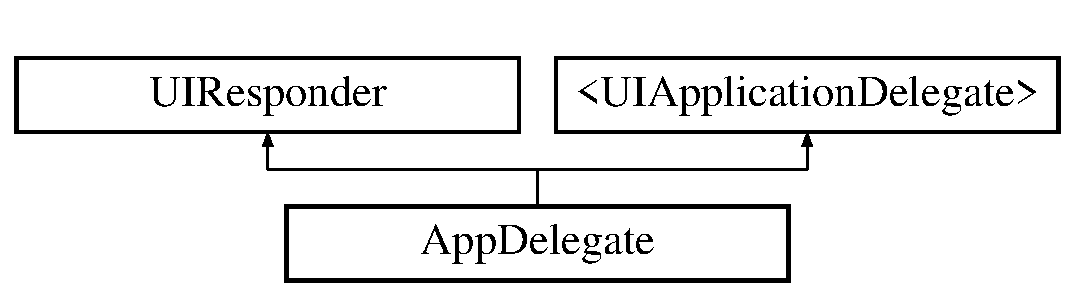
\includegraphics[height=2.000000cm]{interface_app_delegate}
\end{center}
\end{figure}
\subsection*{Properties}
\begin{DoxyCompactItemize}
\item 
\hypertarget{interface_app_delegate_acf48ac24125e688cac1a85445cd7fac2}{U\+I\+Window $\ast$ {\bfseries window}}\label{interface_app_delegate_acf48ac24125e688cac1a85445cd7fac2}

\end{DoxyCompactItemize}


The documentation for this class was generated from the following file\+:\begin{DoxyCompactItemize}
\item 
App\+Delegate.\+h\end{DoxyCompactItemize}

\hypertarget{category_app_delegate_07_08}{\section{App\+Delegate() Category Reference}
\label{category_app_delegate_07_08}\index{App\+Delegate()@{App\+Delegate()}}
}


The documentation for this category was generated from the following file\+:\begin{DoxyCompactItemize}
\item 
App\+Delegate.\+m\end{DoxyCompactItemize}

\hypertarget{interface_error_message}{\section{Error\+Message Class Reference}
\label{interface_error_message}\index{Error\+Message@{Error\+Message}}
}


{\ttfamily \#import $<$Error\+Message.\+h$>$}

Inheritance diagram for Error\+Message\+:\begin{figure}[H]
\begin{center}
\leavevmode
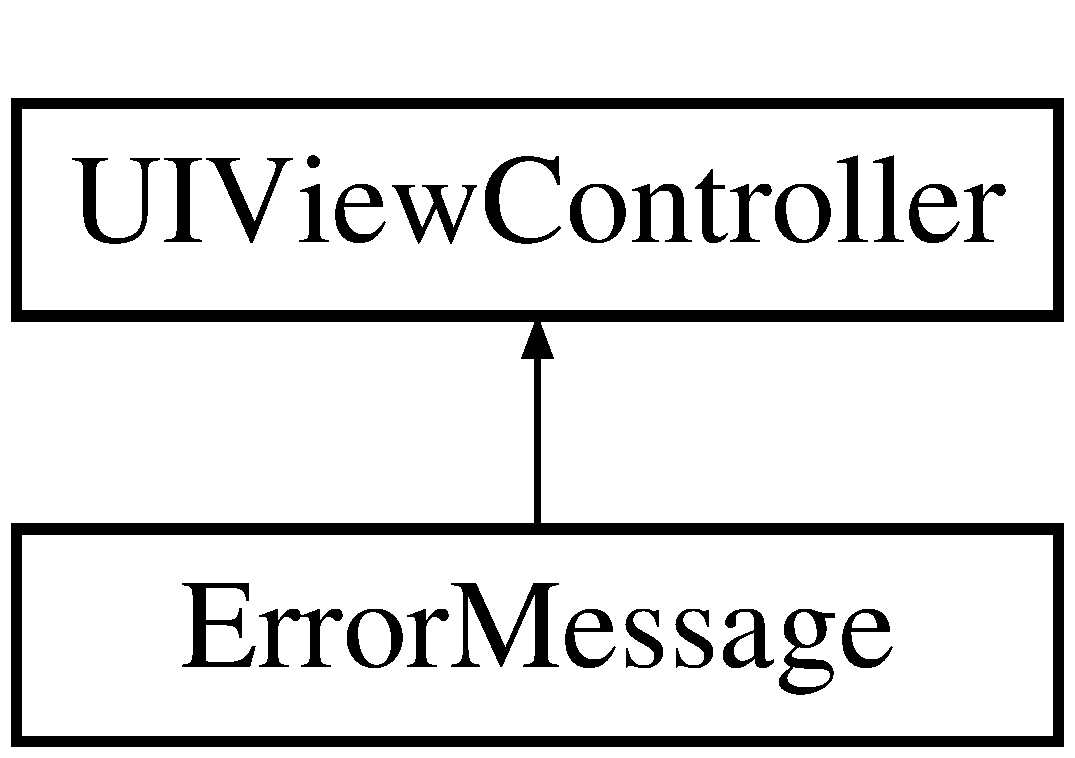
\includegraphics[height=2.000000cm]{interface_error_message}
\end{center}
\end{figure}
\subsection*{Instance Methods}
\begin{DoxyCompactItemize}
\item 
(void) -\/ \hyperlink{interface_error_message_a24e086d6802739aca9088c8610a773d5}{error\+Messages\+:}
\end{DoxyCompactItemize}


\subsection{Detailed Description}
The view controller that handles errors from Firebase. 

\subsection{Method Documentation}
\hypertarget{interface_error_message_a24e086d6802739aca9088c8610a773d5}{\index{Error\+Message@{Error\+Message}!error\+Messages\+:@{error\+Messages\+:}}
\index{error\+Messages\+:@{error\+Messages\+:}!Error\+Message@{Error\+Message}}
\subsubsection[{error\+Messages\+:}]{\setlength{\rightskip}{0pt plus 5cm}-\/ (void) error\+Messages\+: 
\begin{DoxyParamCaption}
\item[{(N\+S\+Error$\ast$)}]{error}
\end{DoxyParamCaption}
}}\label{interface_error_message_a24e086d6802739aca9088c8610a773d5}
Determines error message to display 
\begin{DoxyParams}{Parameters}
{\em error} & is the error code from Firebase\\
\hline
\end{DoxyParams}
These errors are the only errors which can occur during the project, and 

The documentation for this class was generated from the following files\+:\begin{DoxyCompactItemize}
\item 
Error\+Message.\+h\item 
Error\+Message.\+m\end{DoxyCompactItemize}

\hypertarget{interface_forgot_password_view_controller}{\section{Forgot\+Password\+View\+Controller Class Reference}
\label{interface_forgot_password_view_controller}\index{Forgot\+Password\+View\+Controller@{Forgot\+Password\+View\+Controller}}
}


{\ttfamily \#import $<$Forgot\+Password\+View\+Controller.\+h$>$}

Inheritance diagram for Forgot\+Password\+View\+Controller\+:\begin{figure}[H]
\begin{center}
\leavevmode
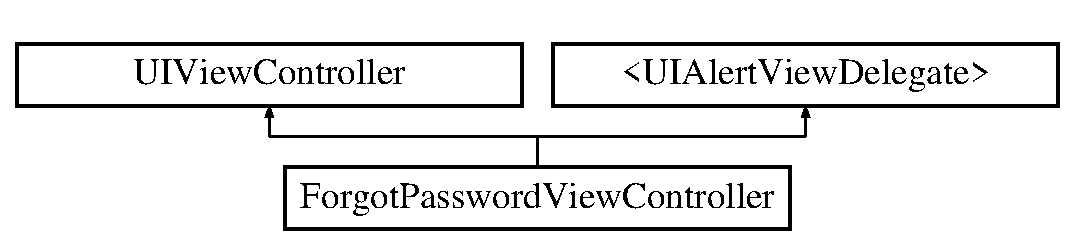
\includegraphics[height=2.000000cm]{interface_forgot_password_view_controller}
\end{center}
\end{figure}
\subsection*{Properties}
\begin{DoxyCompactItemize}
\item 
\hypertarget{interface_forgot_password_view_controller_a2027b91c7f7d7c18817fb441f41686ef}{I\+B\+Outlet U\+I\+Text\+Field $\ast$ \hyperlink{interface_forgot_password_view_controller_a2027b91c7f7d7c18817fb441f41686ef}{email\+Text\+Field}}\label{interface_forgot_password_view_controller_a2027b91c7f7d7c18817fb441f41686ef}

\begin{DoxyCompactList}\small\item\em The field where user enters email. \end{DoxyCompactList}\item 
\hypertarget{interface_forgot_password_view_controller_a935d59e7247b5f17d578a2c3cc27a318}{I\+B\+Outlet U\+I\+Button $\ast$ \hyperlink{interface_forgot_password_view_controller_a935d59e7247b5f17d578a2c3cc27a318}{send\+Email\+Button}}\label{interface_forgot_password_view_controller_a935d59e7247b5f17d578a2c3cc27a318}

\begin{DoxyCompactList}\small\item\em The button that sends password reset. \end{DoxyCompactList}\end{DoxyCompactItemize}


\subsection{Detailed Description}
The view controller to help users send a password reset. 

The documentation for this class was generated from the following file\+:\begin{DoxyCompactItemize}
\item 
Forgot\+Password\+View\+Controller.\+h\end{DoxyCompactItemize}

\hypertarget{interface_login_sign_up}{\section{Login\+Sign\+Up Class Reference}
\label{interface_login_sign_up}\index{Login\+Sign\+Up@{Login\+Sign\+Up}}
}


{\ttfamily \#import $<$Login\+Sign\+Up.\+h$>$}

Inheritance diagram for Login\+Sign\+Up\+:\begin{figure}[H]
\begin{center}
\leavevmode
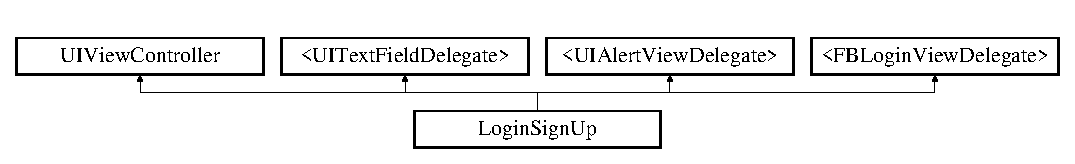
\includegraphics[height=1.761006cm]{interface_login_sign_up}
\end{center}
\end{figure}
\subsection*{Instance Methods}
\begin{DoxyCompactItemize}
\item 
(B\+O\+O\+L) -\/ \hyperlink{interface_login_sign_up_ae3df154525f230ce1e5575d2d10840e2}{validate\+Email\+:}
\item 
(void) -\/ \hyperlink{interface_login_sign_up_a9f5f1dbe36810fd050c96b99935940b4}{standard\+Login\+:with\+Password\+:with\+Created\+:}
\item 
(I\+B\+Action) -\/ \hyperlink{interface_login_sign_up_a3edc0364b4ae4e6a47e798593ebea03d}{unwind\+To\+Login\+Screen\+:}
\end{DoxyCompactItemize}
\subsection*{Properties}
\begin{DoxyCompactItemize}
\item 
\hypertarget{interface_login_sign_up_a797d5135d8e0f5c3764e6c8e863628e8}{I\+B\+Outlet U\+I\+View $\ast$ \hyperlink{interface_login_sign_up_a797d5135d8e0f5c3764e6c8e863628e8}{email\+View}}\label{interface_login_sign_up_a797d5135d8e0f5c3764e6c8e863628e8}

\begin{DoxyCompactList}\small\item\em The view for selecting email login/signup. \end{DoxyCompactList}\item 
\hypertarget{interface_login_sign_up_a9e3a9ddb0ec8c4770478e8e96691aa70}{I\+B\+Outlet U\+I\+View $\ast$ \hyperlink{interface_login_sign_up_a9e3a9ddb0ec8c4770478e8e96691aa70}{options\+View}}\label{interface_login_sign_up_a9e3a9ddb0ec8c4770478e8e96691aa70}

\begin{DoxyCompactList}\small\item\em The view for selecting which login/signup. \end{DoxyCompactList}\item 
\hypertarget{interface_login_sign_up_aef2c833e97693b442b9bf988f7809826}{I\+B\+Outlet U\+I\+Text\+Field $\ast$ \hyperlink{interface_login_sign_up_aef2c833e97693b442b9bf988f7809826}{email\+Text\+Field}}\label{interface_login_sign_up_aef2c833e97693b442b9bf988f7809826}

\begin{DoxyCompactList}\small\item\em The field where users enter email. \end{DoxyCompactList}\item 
\hypertarget{interface_login_sign_up_aad42d499881b619e94e5bbab8b20ce40}{I\+B\+Outlet U\+I\+Text\+Field $\ast$ \hyperlink{interface_login_sign_up_aad42d499881b619e94e5bbab8b20ce40}{password\+Text\+Field}}\label{interface_login_sign_up_aad42d499881b619e94e5bbab8b20ce40}

\begin{DoxyCompactList}\small\item\em The field where users enter his/her password. \end{DoxyCompactList}\item 
\hypertarget{interface_login_sign_up_abee440735a89803ee5a32787941dafe6}{I\+B\+Outlet U\+I\+Text\+Field $\ast$ \hyperlink{interface_login_sign_up_abee440735a89803ee5a32787941dafe6}{username\+Text\+Field}}\label{interface_login_sign_up_abee440735a89803ee5a32787941dafe6}

\begin{DoxyCompactList}\small\item\em Username prompt for first time users. \end{DoxyCompactList}\item 
\hypertarget{interface_login_sign_up_ad834f5c1778788ef1e52a3f293428e0e}{I\+B\+Outlet U\+I\+Button $\ast$ \hyperlink{interface_login_sign_up_ad834f5c1778788ef1e52a3f293428e0e}{forgot\+Password\+Button}}\label{interface_login_sign_up_ad834f5c1778788ef1e52a3f293428e0e}

\begin{DoxyCompactList}\small\item\em Button that allows users to reset password when loggin in. \end{DoxyCompactList}\end{DoxyCompactItemize}


\subsection{Detailed Description}
The view controller for selecting whether logging in or signing up manually or with social network. 

\subsection{Method Documentation}
\hypertarget{interface_login_sign_up_a9f5f1dbe36810fd050c96b99935940b4}{\index{Login\+Sign\+Up@{Login\+Sign\+Up}!standard\+Login\+:with\+Password\+:with\+Created\+:@{standard\+Login\+:with\+Password\+:with\+Created\+:}}
\index{standard\+Login\+:with\+Password\+:with\+Created\+:@{standard\+Login\+:with\+Password\+:with\+Created\+:}!Login\+Sign\+Up@{Login\+Sign\+Up}}
\subsubsection[{standard\+Login\+:with\+Password\+:with\+Created\+:}]{\setlength{\rightskip}{0pt plus 5cm}-\/ (void) standard\+Login\+: 
\begin{DoxyParamCaption}
\item[{(N\+S\+String $\ast$)}]{email}
\item[{withPassword:(N\+S\+String $\ast$)}]{password}
\item[{withCreated:(B\+O\+O\+L)}]{just\+Created}
\end{DoxyParamCaption}
}}\label{interface_login_sign_up_a9f5f1dbe36810fd050c96b99935940b4}
Standard login. Will be called for a normal login including after account creation Will use data to set user defaults. \hypertarget{interface_login_sign_up_a3edc0364b4ae4e6a47e798593ebea03d}{\index{Login\+Sign\+Up@{Login\+Sign\+Up}!unwind\+To\+Login\+Screen\+:@{unwind\+To\+Login\+Screen\+:}}
\index{unwind\+To\+Login\+Screen\+:@{unwind\+To\+Login\+Screen\+:}!Login\+Sign\+Up@{Login\+Sign\+Up}}
\subsubsection[{unwind\+To\+Login\+Screen\+:}]{\setlength{\rightskip}{0pt plus 5cm}-\/ (I\+B\+Action) unwind\+To\+Login\+Screen\+: 
\begin{DoxyParamCaption}
\item[{(U\+I\+Storyboard\+Segue $\ast$)}]{segue}
\end{DoxyParamCaption}
}}\label{interface_login_sign_up_a3edc0364b4ae4e6a47e798593ebea03d}
Allows mobility to move back to login screen. \hypertarget{interface_login_sign_up_ae3df154525f230ce1e5575d2d10840e2}{\index{Login\+Sign\+Up@{Login\+Sign\+Up}!validate\+Email\+:@{validate\+Email\+:}}
\index{validate\+Email\+:@{validate\+Email\+:}!Login\+Sign\+Up@{Login\+Sign\+Up}}
\subsubsection[{validate\+Email\+:}]{\setlength{\rightskip}{0pt plus 5cm}-\/ (B\+O\+O\+L) validate\+Email\+: 
\begin{DoxyParamCaption}
\item[{(N\+S\+String $\ast$)}]{candidate}
\end{DoxyParamCaption}
}}\label{interface_login_sign_up_ae3df154525f230ce1e5575d2d10840e2}
catlan stack\+O\+F \href{http://stackoverflow.com/questions/800123/what-are-best-practices-for-validating-email-addresses-in-objective-c-for-ios-2/1149894#1149894}{\tt http\+://stackoverflow.\+com/questions/800123/what-\/are-\/best-\/practices-\/for-\/validating-\/email-\/addresses-\/in-\/objective-\/c-\/for-\/ios-\/2/1149894\#1149894} a regular expression that regulates what user emails can create. W\+I\+L\+L accept crazy emails !matt\$=\href{mailto:awesome@mail.aol.biz}{\tt awesome@mail.\+aol.\+biz} 

The documentation for this class was generated from the following files\+:\begin{DoxyCompactItemize}
\item 
Login\+Sign\+Up.\+h\item 
Login\+Sign\+Up.\+m\end{DoxyCompactItemize}

\hypertarget{interface_login_sign_up_tests}{\section{Login\+Sign\+Up\+Tests Class Reference}
\label{interface_login_sign_up_tests}\index{Login\+Sign\+Up\+Tests@{Login\+Sign\+Up\+Tests}}
}
Inheritance diagram for Login\+Sign\+Up\+Tests\+:\begin{figure}[H]
\begin{center}
\leavevmode
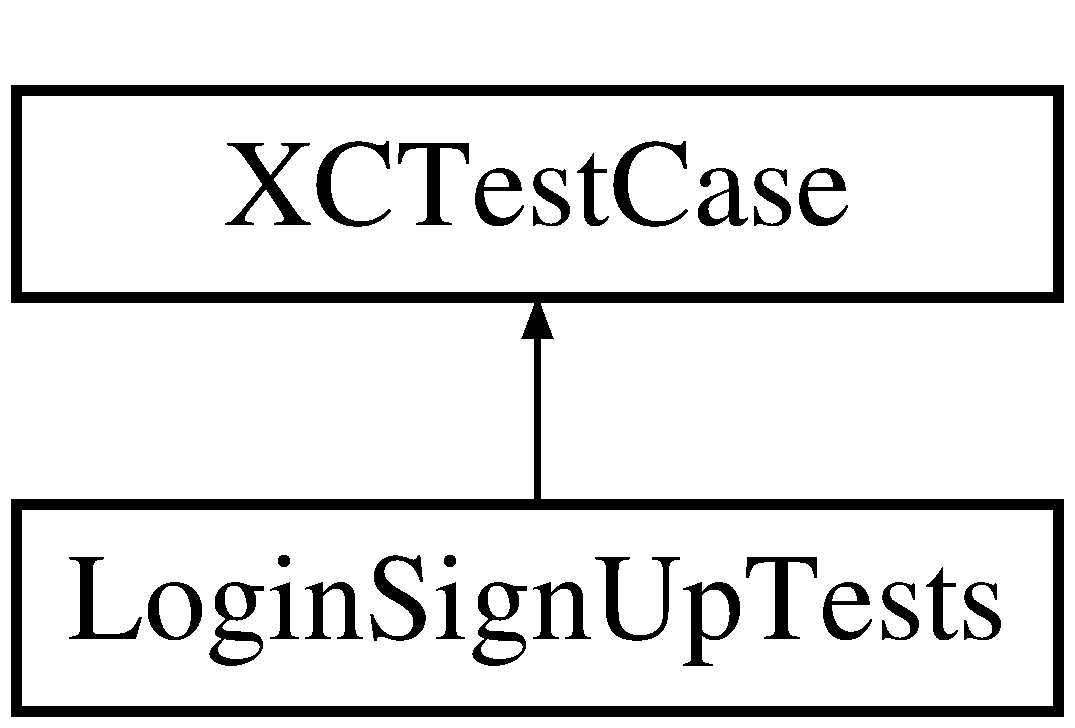
\includegraphics[height=2.000000cm]{interface_login_sign_up_tests}
\end{center}
\end{figure}


The documentation for this class was generated from the following file\+:\begin{DoxyCompactItemize}
\item 
Login\+Sign\+Up\+Tests.\+m\end{DoxyCompactItemize}

%--- End generated contents ---

% Index
\newpage
\phantomsection
\addcontentsline{toc}{chapter}{Index}
\printindex

\end{document}
